\documentclass[11pt]{article}
\usepackage[utf8]{inputenc}	% Para caracteres en español
\usepackage{amsmath,amsthm,amsfonts,amssymb,amscd}
\usepackage{multirow,booktabs}
\usepackage[table]{xcolor}
\usepackage{fullpage}
\usepackage{lastpage}
\usepackage{enumitem}
\usepackage{fancyhdr}
\usepackage{mathrsfs}
\usepackage{wrapfig}
\usepackage{setspace}
\usepackage{siunitx}
\usepackage{svg}
\usepackage{calc}
\usepackage{multicol}
\usepackage{cancel}
\usepackage[retainorgcmds]{IEEEtrantools}
\usepackage[margin=3cm]{geometry}
\usepackage{amsmath}
\newlength{\tabcont}
\setlength{\parindent}{0.0in}
\setlength{\parskip}{0.05in}
\usepackage{physics}
\usepackage{empheq}
\usepackage{framed}
\usepackage[most]{tcolorbox}
\usepackage{xcolor}
\usepackage{tikz}
\usepackage{tikz-3dplot}
\usepackage{pgfplots}
\pgfplotsset{width=10cm,compat=1.9}
\usepgfplotslibrary{external}
\tikzexternalize

\colorlet{shadecolor}{orange!15}
\parindent 0in
\parskip 12pt
\geometry{margin=1in, headsep=0.25in}
\theoremstyle{definition}
\newtheorem{defn}{Definition}
\newtheorem{reg}{Rule}
\newtheorem{exer}{Exercise}
\newtheorem{note}{Note}
\begin{document}
\setcounter{section}{8}
\title{Chapter 9 Review Notes}

\thispagestyle{empty}

\begin{center}
{\LARGE \bf Quantum Chemistry}\\
{\large CML101}\\
Salil Gokhale
\end{center}

\section{Postulates of Quantum Mechanics}
\subsection{Postulate I: The Wavefunction}

\textbf{The state of the system is described as fully as possible by the wavefunction $\psi(r_1, r_2,\dots ,t)$ where $r_1$, $r_2, \dots$ are the locations of the particles and $t$ is time.}

$\psi(r_1, r_2,\dots ,t) \rightarrow$ time-dependent wavefunction

$\psi(r_1, r_2,\dots) \rightarrow$ time-independent wavefunction

\subsubsection{Born Interpretation} 
\textbf{For a system described by the wavefunction $\psi(r_1, r_2, \dots)$ the probability of finding particle 1 in the volume element $\dd{\tau_1}$ at $r_1$, particle 2 in the volume element $\dd{\tau_2}$ at $r_2$, etc. is proportional to $\abs{\psi}^2 \dd{\tau_1} \dd{\tau_2} \dots$}

$\abs{\psi}^2 \rightarrow$ probability density

$\psi \rightarrow$ probability amplitude. It has no physical significance 

\subsubsection{Normalisation Condition} 

A wavefunction is said to be normalised if $\int \psi^* \psi \dd{\tau} =1$

Hence the normalisation constant $N$(which when multiplied to the wavefunction normalises it) is equal to $\frac{1}{\left(\int \psi^* \psi \dd{\tau} \right)^{1/2}}$. If this integral has a finite value, the wavefunction is \textbf{square-integrable}.

\subsubsection{Constraints on Wavefunction}

\begin{itemize}
    \item $\psi$ must not be infinite over a finite region
    \item $\psi$ must be single-valued
    \item $\psi$ must be continuous
    \item $\dv{\psi}{x}$ must be continuous
\end{itemize}


\subsection{Postulate II: Quantum Mechanical Operators}

\textbf{For each observable property $\Omega$ of a system there is a corresponding operator $\vectorunit{\Omega}$ built from the following position and momentum operators:}

\begin{itemize}
    \item $\vectorunit{x} = x \times$
    \item $\vectorunit{p} = -i \hbar \grad$ or in special case of one dimension $\vectorunit{p}_x = -i\hbar \pdv{x}$
\end{itemize}

All the operators we encounter are linear i.e. $\vectorunit{\Omega}(\psi_1 + \psi_2) =  \vectorunit{\Omega}(\psi_1) + \vectorunit{\Omega}(\psi_2)$

\begin{shaded}
\textbf{Time-independent Schrodinger Equation}
\begin{equation*}
\vectorunit{H}\psi = E\psi
\end{equation*}

where,

\begin{gather*}
\vectorunit{H} = \frac{-\hbar^2}{2m} \laplacian + V \text{ is the hamiltonian operator corresponding to total energy of system.} \\
E \text{ is the total energy of system}
\end{gather*}
\end{shaded}



This suggests the form of the \textbf{eigenvalue equation} 

\begin{equation*}
    \vectorunit{\Omega} \psi = \omega \psi
\end{equation*}

where,
\begin{gather*}
    \vectorunit{\Omega} \text{ is a operator corresponding to an observable} \\
    \omega\text{ is called observable or \textbf{eigenvalue} of operator. It is always a real value.}\\
    \psi \text{ is the wavefunction and also called as \textbf{eigenfunction} of the operator}
\end{gather*}

\subsection{Postulate III: Eigenvalues and Eigenfunctions}
\textbf{If the system is described by a wavefunction $\psi$ that is an eigenfunction of $\vectorunit{\Omega}$ such that $\vectorunit{\Omega} \psi = \omega \psi$ then the outcome of a measurement of $\Omega$ will be the eigenvalue $\omega$.Operator $\vectorunit{\Omega}$ has to be Hermitian and observable $\omega$ has to be purely real.}


\begin{equation*}
    \int \psi_1 ^* \vectorunit{\Omega} \psi_2 \dd{x} = \left[ \int \psi_2 ^* \vectorunit{\Omega} \psi_1 \dd{x} \right]^* \quad \quad \forall \psi_1, \psi_2
\end{equation*}
The momentum and position operators are hermitian. Sum and product of two hermitian operators is also hermitian.

\subsubsection{Orthogonality of Eigenfunctions}
\textbf{Eigenfunctions corresponding to different eigenvalues of the same Hermitian operator are orthogonal.} To say that two different functions $\psi_i$ and $\psi_j$ are orthogonal means that the integral (over all space) of their product is zero:

\begin{equation*}
    \int \psi_i ^* \psi_j \dd{\tau} = 0
\end{equation*}
in a special case when both functions are normalised,

\begin{equation*}
    \int \psi_i ^* \psi_j \dd{\tau} = \delta_{ij}
\end{equation*}

\subsection{Postulate IV: Basis Set Postulate}

\textbf{The set of functions $\psi_k$ which are eigenfunctions of the eigenvalue equation form a complete set of linearly independent functions. They can be said to form a basis set in terms of which any wavefunction representing the system can be expressed:}
\begin{equation*}
    \psi = \sum_{k=1}^{\infty} c_k \psi_k
\end{equation*}

This implies that any wavefunction $\psi$ representing a physical system can be expressed as a linear combination of the eigenfunctions of any physical observable of the system. This is the Fourier Series of $\psi$ and it's existence is ensured by Dirichlet's Theorem. You can find the constant $c_m$ by Fourier's trick: Multiply both sides by some $\psi_m^*$ and integrate.

$$\int_0 ^{\infty} \psi_m^* \psi \dd{x} = \sum_{k=1} ^{\infty} c_k\int_0 ^{\infty} \psi_m^* \psi_k \dd{x} =  \sum_{k=1} ^{\infty} c_k \delta_{m, k} = c_m$$

$$\therefore c_m = \int_0 ^{\infty} \psi_m^* \psi \dd{x} $$



\subsection{Postulate V: Predicting Experiments}
\textbf{When the value of an observable $\Omega$ is measured for a system that is described by a wavefunction which is a linear combination, $\psi = \sum_k c_k \psi_k$, each measurement of $\Omega$ gives one of the eigenvalues $\omega_k$ with a probability proportional to $\abs{c_k}^2$.}
If $\psi$ is normalised, then this probability is equal to $\abs{c_k}^2$.


\begin{shaded}
The mean of the measurements of $\Omega$ is equal to expectation value of the operator $\vectorunit{\Omega}$

\begin{equation*}
    \expval{\Omega} = \frac{\int \psi^* \vectorunit{\Omega} \psi \dd{\tau}}{\int \psi^* \psi \dd{\tau}}
\end{equation*}
for a normalised wavefunction, the denominator is unity. If $\psi$ is an eigenfunction of $\vectorunit{\Omega}$ then each measurement and consequently expectation value will be equal to it's eigenvalue $\omega$.

In the case of $\psi = \sum_{k} c_k \psi_k$, the expectation value is($\psi$ is normalised)
\begin{equation*}
    \expval{\Omega} = \sum_{k} \abs{c_k}^2 \omega_k
\end{equation*}

\end{shaded}




\section{The Uncertainty Principle}
\begin{shaded}
\textbf{Heisenberg Uncertainty Principle}
\begin{equation*}
    \Delta p_x \Delta x \geq \frac{\hbar}{2}
\end{equation*}
where,
\begin{gather*}
     \Delta X = \left[\expval{X^2} - \expval{X}^2 \right]^{1/2}
\end{gather*}

Note that there is no such constraint on say, $p_y$ and $x$
\end{shaded}

\subsection{General Form of Uncertainty principle}

Two observables $\Omega_1$ and $\Omega_2$ are complementary if $\vectorunit{\Omega}_1 \vectorunit{\Omega}_2 \psi \neq  \vectorunit{\Omega}_2 \vectorunit{\Omega}_1 \psi$

The commutator of the two operators is defined as their difference: $\comm{\vectorunit{\Omega}_1}{\vectorunit{\Omega}_2} = \vectorunit{\Omega}_1\vectorunit{\Omega}_2 - \vectorunit{\Omega}_2\vectorunit{\Omega}_1$. If two operators commute then their commutator is 0.

\begin{shaded}
\textbf{General Uncertainty Principle}
\begin{equation*}
    (\Delta \Omega_1)^2 (\Delta \Omega_2)^2 \geq \left(\frac{1}{2i}\expval{ \comm{\vectorunit{\Omega}_1}{\vectorunit{\Omega}_2}}\right)^2
\end{equation*}
from which it immediately follows that
\begin{equation*}
    \Delta \Omega_1 \Delta \Omega_2 \geq \abs{\frac{1}{2i} \expval{ \comm{\vectorunit{\Omega}_1}{\vectorunit{\Omega}_2}}}
\end{equation*}
\end{shaded}




\section{Motion in 1D}

A particle with net motion is described by a complex wavefunction. A wavefunction that is purely real corresponds to zero net motion. Because purely real wavefunction can be described as a linear combination of wavefunctions which are conjugates of each other. This gives an expectation value of 0 to linear momentum

For a freely moving particle in one dimension, Schrodinger's equation is

\begin{shaded}
\begin{equation*}
    - \frac{\hbar}{2m} \dv[2]{\psi(x)}{x} = E \psi(x)
\end{equation*}

Solving this we get the general solutions as,

\begin{gather*}
    \psi_k = Ae^{ikx} + Be^{-ikx}\\
    E_k = \frac{k^2 \hbar^2}{2m}
\end{gather*}
\end{shaded}

It follows that in this case, energy is \textbf{not} quantized.

\subsection{Particle in a 1D box}

Particle is confined between $x=0$ and $x=L$. Hence potential energy is:
\begin{equation*}
V=\begin{cases}
          0 \quad &\text{if } \, x \in (0,L) \\
          \infty \quad &\text{if } \, x \in (-\infty,0] \cup [L, \infty) \\
     \end{cases}
\end{equation*}

For particle inside walls, wavefunction will be same as that for free motion. It would be more convenient to write $\psi_k =Ae^{ikx} + Be^{-ikx}$ as $\psi_k = C\sin{kx} + D \cos{kx}$ where $C = (A-B)i$, $D = (A+B)$. For particle outside walls, wavefunction is 0.

\begin{equation*}
\psi_k(x) =\begin{cases}
          C\sin{kx} + D \cos{kx} \quad &\text{if } \, x \in (0,L) \\
          0 \quad &\text{if } \, x \in (-\infty,0] \cup [L, \infty) \\
     \end{cases}
\end{equation*}
At the moment, it seems that $k$ can take any value.

\subsubsection{Restricting values of $k$}

For continuity of wavefunction, it must satisfy the following boundary conditions:
\begin{itemize}
    \item $\psi_k (0) = 0$
    \item $\psi_k (L) = 0$
\end{itemize}

First condition implies that $D=0$ and second condition implies $k = \frac{n\pi}{L}$. normalising the wavefunction gives $C = \left(\frac{2}{L}\right)^{1/2}$. This will quantize the system by allowing only discrete values.
\begin{shaded}
\begin{equation*}
\psi_n(x) =\begin{cases}
          \left(\frac{2}{L}\right)^{1/2}\sin{\frac{n\pi x}{L}} \quad &\text{if } \, x \in (0,L) \\
          0 \quad &\text{if } \, x \in (-\infty,0] \cup [L, \infty) \\
     \end{cases}
\end{equation*}
and 
\begin{equation*}
    E_n = \frac{n^2 \pi^2 \hbar^2}{2mL^2} = \frac{n^2 h^2}{8mL^2} \quad  \text{ where }n=1,2,3,\dots
\end{equation*}
\end{shaded}
\subsubsection{Properties of Wavefunction}
\textbf{Nodes are points where the wavefunction passes through zero (not merely reaching zero, as at the walls)}. This particular wavefunction has $n-1$ nodes.

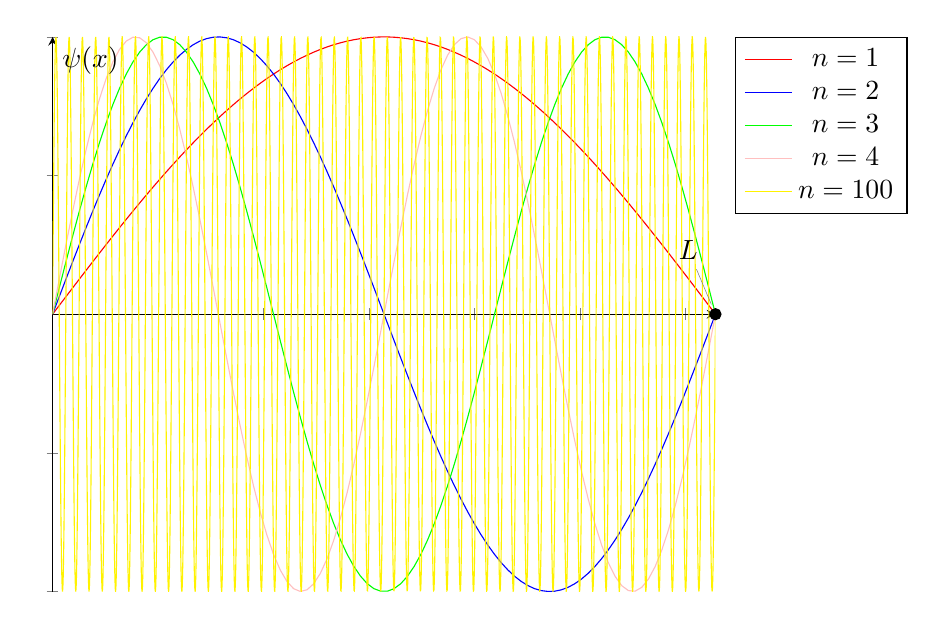
\begin{tikzpicture}
\begin{axis}[
    axis lines = center,
    ylabel = {\(\psi(x)\)},
    yticklabels={,,},
    xticklabels={,,},
    legend pos=outer north east,
]

\addplot [
    domain=0:pi, 
    samples=100, 
    color=red,
]
{sin(deg(x))};
\addlegendentry{\(n=1\)}

\addplot [
    domain=0:pi, 
    samples=100, 
    color=blue,
]
{sin(deg(2*x))};
\addlegendentry{\(n=2\)}

\addplot [
    domain=0:pi, 
    samples=100, 
    color=green,
]
{sin(deg(3*x))};
\addlegendentry{\(n=3\)}

\addplot [
    domain=0:pi, 
    samples=100, 
    color=pink,
]
{sin(deg(4*x))};
\addlegendentry{\(n=4\)}

\addplot [
    domain=0:pi, 
    samples=2000, 
    color=yellow,
]
{sin(deg(100*x))};
\addlegendentry{\(n=100\)}

\addplot[mark=*] coordinates {(pi,0)} node[pin=100:{$L$}]{} ;

\end{axis}
\end{tikzpicture}

The probability density $\psi^2(x)$ becomes more uniform as $n$ increases, provided we ignore the fine detail of the increasingly rapid oscillations. The probability density at high quantum numbers reflects the classical result that a particle bouncing between the walls spends, on the average, equal times at all points. Thus classical mechanics emerges from quantum mechanics as high quantum numbers are reached.
\subsubsection{Properties of Observables}

$$\psi_n(x) = \left(\frac{2}{L}\right)^{1/2}\sin{\frac{n\pi x}{L}} = \frac{1}{2i}\left(\frac{2}{L}\right)^{1/2} (e^{ikx} + e^{-ikx})$$
It follows that linear momentum will be $k\hbar$ for half measurements and $-k\hbar$ for other half. So expectation value is 0. Which we could even obtain directly by integration:

\begin{equation*}
    \expval{p} =  \frac{-2 i\hbar n \pi}{L^2} \int_0 ^L \sin{\frac{n\pi x}{L}} \cos{\frac{n \pi x}{L}} \dd{x} = 0
\end{equation*}

Because $n$ cannot be zero, the lowest energy that the particle may possess is not zero (as would be allowed by classical mechanics) but this lowest, irremovable energy is called the \textbf{zero-point energy}. The physical origin of the zero-point energy can be explained in two ways:

\begin{itemize}
    \item The Heisenberg uncertainty principle requires a particle to possess kinetic energy if it is confined to a finite region(which in this case is true)
    \item If the wavefunction is to be zero at the walls, but smooth, continuous, and not zero everywhere, then it must be curved, and curvature in a wavefunction implies the possession of kinetic energy.
\end{itemize}
\section{Motion in 2D and 3D}
\subsection{Motion in 2D box}
Let the region of box be $\{(x,y) \mid 0<x<L_1, 0<y<L_2 \}$.
Schrodinger's equation will be 

\begin{equation*}
    \frac{-\hbar^2}{2m} \left(\dv[2]{\psi}{x} + \dv[2]{\psi}{y}\right) = E \psi
\end{equation*}

\subsubsection{Separation of Variables}

Assume that $\psi$ can be written as a product of two function $X(x)$ and $Y(y)$. I.e. $\psi(x,y) = X(x) Y(y)$.

Substituting this in Schrodinger's equation, dividing both sides by $XY$ and rearranging,
\begin{equation*}
    \frac{1}{X}\dv[2]{X}{x} + \frac{1}{Y} \dv[2]{Y}{y} = -\frac{2mE}{\hbar^2}
\end{equation*}
The first term on the left is independent of $y$, so if $y$ is varied only the second term of the two on the left can change. But the sum of these two terms is a constant given by the right-hand side of the equation. Hence both the terms of left are constants. We can then break it like this:

\begin{gather*}
    \frac{1}{X}\dv[2]{X}{x} =-\frac{2mE_X}{\hbar^2} \quad \text{and} \quad \frac{1}{Y}\dv[2]{Y}{y} =-\frac{2mE_Y}{\hbar^2}\\
    -\frac{\hbar^2}{2m} \dv[2]{X}{x} = E_X X \quad \text{and} \quad  -\frac{\hbar^2}{2m} \dv[2]{Y}{y} = E_Y Y\\
    \text{where, }\\
    E = E_X + E_Y
\end{gather*}

This is exactly the equation for a particle in 1D box. So we can directly write the wavefunction easily:

\begin{shaded}
\textbf{2D box}
\begin{gather*}
    \psi_{n_1, n_2}(x,y) = \begin{cases}
    \frac{2}{(L_1 L_2)^{1/2}} \sin{\frac{n_1 \pi x}{L_1}} \sin{\frac{n_2 \pi y}{L_2}} \quad \text{for} \quad 0<x<L_1, 0<y<L_2\\
    \\
    0 \quad \text{otherwise}
    \end{cases}
\end{gather*}

Similarly, $E = E_x + E_y$
\begin{equation*}
    E_{n_1, n_2} = \frac{h^2}{8m} \left(\frac{n_1^2}{L_1^2} + \frac{n_2^2}{L_2^2}\right)
\end{equation*}
\end{shaded}

\subsubsection{Degeneracy}

Now consider a situation where $L_1 = L_2 = L$. Then $n_1 = 1, n_2 = 2$ and $n_2 = 1, n_1 = 2$ will yield different wavefunctions but same energy. The technical term for different wavefunctions with same energy is \textbf{degeneracy.} In this case, we say the state is \textbf{double degenerate}. 

Each occurrence of degeneracy is related to a symmetry of the system. In this case it's rotating the box by $90^0$ changes $\psi_{1,2}$ into $\psi_{2,1}$.

\subsubsection{Multiplicity}
\textbf{Multiplicity is defined as $2S+1$ where $S$ is total spin angular momentum quantum number.} Multiplicity tells the number of permitted values of $m_s$, the spin quantum number. For electron in atom, multiplicity $= 2$, because only $m_s = 1/2$ and $m_s = -1/2$ are allowed.

Also these permitted values of spin quantum number are $\{-S, -S+1, -S+2 ,\dots , S \}$
\subsection{Motion in 3D box}

Using similar separation of variables we get the following:
\begin{shaded}
\textbf{3D box}
\begin{gather*}
    \psi_{n_1, n_2, n_3}(x,y,z) = \begin{cases}
    \frac{2\sqrt{2}}{(L_1 L_2 L_3)^{1/2}} \sin{\frac{n_1 \pi x}{L_1}} \sin{\frac{n_2 \pi y}{L_2}} \sin{\frac{n_3 \pi z}{L_3}} \quad \text{for} \quad 0<x<L_1, 0<y<L_2, 0<z<L_3\\
    \\
    0 \quad \text{otherwise}
    \end{cases}
\end{gather*}

Similarly, $E = E_x + E_y + E_z$
\begin{equation*}
    E_{n_1, n_2,n_3} = \frac{h^2}{8m} \left(\frac{n_1^2}{L_1^2} + \frac{n_2^2}{L_2^2} + \frac{n_3^2}{L_3^2d}\right)
\end{equation*}
\end{shaded}

\section{Particle on a Ring}
Let the particle move in a circle of radius $r$ in the $x,y$ plane and having a linear momentum $p$ at some instant. The angular momentum along $z$ axis is $$J_z = \pm pr$$ Let moment of inertia of system be $I$. Then kinetic energy is $$E = \frac{J_z^2}{2I}$$ This equation is valid for any body having moment of inertia $I$ rotating in a plane, not just a particle.


\subsection{Quantised Rotation}

Since $p = h/ \lambda$ by de Broglie relation, we get

\begin{gather*}
    J_z = \pm \frac{hr}{\lambda}\\
    E = \frac{h^2 r^2}{2I\lambda^2}
\end{gather*}

Because wavefunction must be single valued, it must repeat after a complete rotation. Hence, an
integer number of wavelengths must fit the circumference of
the ring.

\begin{equation*}
    n\lambda = 2\pi r \quad , \quad n = 0,1,2,\dots
\end{equation*}

$n=0$ corresponds to $\lambda = \infty$, a wave that has constant height. Applying this constraint to $J_z$ and $E$ gives:

\begin{gather*}
    J_z = \pm \frac{n h}{2\pi} = m_l \hbar \quad, \quad m = 0, \pm 1, \pm 2, \dots \\
    E = \frac{m_l^2 \hbar^2}{2I} \quad , \quad m = 0, \pm 1, \pm 2, \dots
\end{gather*}

A few observations:
\begin{itemize}
    \item States with a given nonzero value of $\abs{m_l}$ are doubly degenerate because of $\pm$.
    \item Only the state described by $m_l = 0$ is non-degenerate, consistent with the interpretation that, when $m_l$ is zero, the particle has an infinite wavelength and is stationary
    \item Each state can be occupied by 2 electrons even for $m_l = 0$
    \item There is no zero-point energy in this system: the lowest possible energy is $E_0 = 0$
\end{itemize}

\subsection{Wavefunction}

Solving the PDE $-\frac{\hbar^2}{2I} \dv[2]{\psi}{\phi} = E\psi$, gives us the state of system

\begin{shaded}
\textbf{Particle on a ring}

\begin{gather*}
    \psi_{m_l}(\phi) = \frac{e^{i m_l \phi}}{(2\pi)^{1/2}}\\
    J_{z} = m_l \hbar \\
    E_{m_l} = \frac{m_l ^2 \hbar^2}{2I}
\end{gather*}

where, $m_l = 0, \pm 1, \pm 2, \dots$
\end{shaded}

\section{Dirac Notation}

\begin{equation*}
    \ket{\psi} = \sum_{i=0}^n a_{i}\ket{\vectorunit{\psi}_i}
\end{equation*}
This is called a \textbf{ket}. It is a column vector with coefficients $a_i$(which may be complex) along the unit basis vectors $\ket{\vectorunit{\psi}_i}$. We can write $\ket{\psi}$ as a column vector:
\begin{equation}
   \ket{\psi}= \mqty[a_1 \\ a_2 \\ \vdots \\ a_n]
\end{equation}

A \textbf{bra} is a row vector which consists of complex conjugates of $a_i$. It is shows as $\bra{\psi}$

\begin{equation}
   \bra{\psi}= \mqty[a_1^* & a_2^* & \dots & a_n^*]
\end{equation}

Scalar product of $\bra{\psi_i}$ and $\ket{\psi_j}$ is just written as $\bra{\psi_i}\ket{\psi_j} = \sum_{i=0}^n a_i^* b_i$. The order of scalar product matters if the coefficients are complex numbers because $\bra{\psi_i}\ket{\psi_j} =  \bra{\psi_j}\ket{\psi_i}^*$

It follows that if the wavefunctions are normalised,  $\bra{\psi_i}\ket{\psi_j} = \delta_{ij}$

\textbf{Because $\bra{\psi}$ and $\ket{\psi}$ exist in different mathematical spaces, we cannot add or subtract them.}

\subsection{Observables and Operators}

The eigenvalue equation can be written as:

\begin{equation*}
    \vectorunit{\Omega} \ket{\psi} = \omega \ket{\psi}
\end{equation*}
where $\psi$ is an \textbf{eigenvector} of $\vectorunit{\Omega}$.

Multiplying both sides by $\bra{\psi}$ gives

\begin{equation*}
    \ev{\vectorunit{\Omega}}{\psi} = \ev{\omega}{\psi} = \omega \bra{\psi}\ket{\psi}
\end{equation*}
because $\omega$ is just a scalar real value. And if $\bra{\psi}$ is normalised, we can easily write the expectation value of $\omega$ in state $\psi$.

\begin{shaded}
\textbf{Expectation Value}
\begin{equation*}
    \expval{\omega}_{\psi} =  \ev{\vectorunit{\Omega}}{\psi} = \int \psi^* \vectorunit{\Omega} \psi \dd{\tau}
\end{equation*}
This is the derivation for expectation value in Postulate V.
\end{shaded}

Properties of operators (some already discussed before):

\begin{itemize}
    \item Operators are linear $\vectorunit{\Omega} (\ket{\psi_1} + \ket{\psi_2}) =\vectorunit{\Omega}  \ket{\psi_1} + \vectorunit{\Omega}\ket{\psi_1} $
    \item Operators with real eigenvalues are Hermitian $\bra{\psi_1}\vectorunit{\Omega}\ket{\psi_2} = \bra{\psi_2}\vectorunit{\Omega}\ket{\psi_1}$
    \item Hermitian operator with a set of eigenvectors which have different eigenvalues are orthogonal $\bra{\psi_i}\ket{\psi_j} = 0$
    \item There exists a set of eigenvectors of both operators $\vectorunit{\Omega}_1$ and $\vectorunit{\Omega}_2$ $\iff$ these operators commute, $\comm{\vectorunit{\Omega}_1}{\vectorunit{\Omega}_2} = 0$
    \begin{shaded}
    \textbf{Proof}
    \begin{gather*}
        \vectorunit{\Omega}_1 \ket{\psi} = \omega_1 \ket{\psi}\\
        \vectorunit{\Omega}_2 \ket{\psi} = \omega_2 \ket{\psi}
    \end{gather*}
    Multiplying first equation by $\vectorunit{\Omega}_2$ and second equation by $\vectorunit{\Omega}_1$ gives,
    \begin{gather*}
        \vectorunit{\Omega}_2 \vectorunit{\Omega}_1 \ket{\psi} = \omega_1 \vectorunit{\Omega}_2 \ket{\psi} = \omega_1 \omega_2 \ket{\psi}\\
        \vectorunit{\Omega}_1 \vectorunit{\Omega}_2 \ket{\psi} = \omega_2 \vectorunit{\Omega}_1 \ket{\psi} = \omega_2 \omega_1 \ket{\psi}\\
    \end{gather*}
    
    Subtracting them gives the required result.
    \end{shaded}
\end{itemize}

\section{Hydrogenic Atom}
Schrodinger Equation in cartesian will be(we assume that nucleus is at rest and only electrostatic interactions are present):

\begin{equation*}
    -\frac{\hbar^2}{2m_e} \grad^2 \psi -\frac{Ze^2}{4\pi \epsilon_0 \sqrt{x^2 + y^2 + z^2}} = E\psi 
\end{equation*}
We cannot solve this PDE, hence we switch to spherical coordinates

%Axis Angles  
\tdplotsetmaincoords{70}{110}

%Macros  
\pgfmathsetmacro{\rvec}{6}  
\pgfmathsetmacro{\thetavec}{40}  
\pgfmathsetmacro{\phivec}{45}

\pgfmathsetmacro{\dphivec}{20}  
\pgfmathsetmacro{\dthetavec}{20}  
\pgfmathsetmacro{\drvec}{1.5}

%Layers  
\pgfdeclarelayer{background} 
\pgfdeclarelayer{foreground}

\pgfsetlayers{background, main, foreground}

\begin{tikzpicture}[tdplot_main_coords]

%Coordinates  
\coordinate (O) at (0,0,0);  
\tdplotsetcoord{A}{\rvec}{\thetavec}{\phivec}  
\tdplotsetcoord{B}{\rvec}{\thetavec + \dthetavec}{\phivec}         
\tdplotsetcoord{C}{\rvec}{\thetavec + \dthetavec}{\phivec + \dphivec}  
\tdplotsetcoord{D}{\rvec}{\thetavec}{\phivec + \dphivec}  
\tdplotsetcoord{E}{\rvec + \drvec}{\thetavec}{\phivec}  
\tdplotsetcoord{F}{\rvec + \drvec}{\thetavec + \dthetavec}{\phivec}  
\tdplotsetcoord{F'}{\rvec + \drvec}{90}{\phivec}  \tdplotsetcoord{G}{\rvec + \drvec}{\thetavec + \dthetavec}{\phivec + \dphivec}  
\tdplotsetcoord{G'}{\rvec + \drvec}{90}{\phivec + \dphivec} 
\tdplotsetcoord{H}{\rvec + \drvec}{\thetavec}{\phivec + \dphivec} 
    
%Axis  
\begin{pgfonlayer}{background}  
    \draw[thick,-latex] (0,0,0) -- (7,0,0) node[pos=1.1]{$x = r\sin{\theta} \cos{\phi}$};        
    \draw[thick,-latex] (0,0,0) -- (0,7,0) node[pos=1.15]{$y = r\sin{\theta} \sin{\phi}$};         
    \draw[thick,-latex] (0,0,0) -- (0,0,6) node[pos=1.05]{$z = r\cos{\theta}$};                   
\end{pgfonlayer}

%Help Lines  
\begin{pgfonlayer}{background}  
    %Up     
    \draw[thick, blue] (O) -- (A) node[pos=0.6, above left, red] {$r$};    
    \draw [blue](O) -- (B);   
    \draw [blue](O) -- (C);   
    \draw[dashed,blue] (O) -- (D);   
    %Down   
    \draw (O) -- (F');  
    \draw (O) -- (G');  
\end{pgfonlayer}  
\begin{pgfonlayer}{foreground}  
    %%Help Curves   
    \tdplotsetthetaplanecoords{\phivec}     
    \tdplotdrawarc[tdplot_rotated_coords]{(O)}{\rvec}{\thetavec+\dthetavec}{90}{}{}
    %
    \tdplotdrawarc[tdplot_rotated_coords]{(O)}{\rvec+\drvec}{\thetavec+\dthetavec}{90}{}{}
    %
    \tdplotsetthetaplanecoords{\phivec+\dphivec}    
    \tdplotdrawarc[tdplot_rotated_coords, dashed]{(O)}{\rvec}{\thetavec+\dthetavec}{90}{}{}     
    \tdplotdrawarc[tdplot_rotated_coords]{(O)}{\rvec+\drvec}{\thetavec+\dthetavec}{90}{}{}
    %   
    \tdplotdrawarc[tdplot_main_coords]{(O)}{\rvec}{\phivec}{\phivec+\dphivec}{}{}
    %    
    \tdplotdrawarc[tdplot_main_coords]{(O)}{\rvec+\drvec}{\phivec}{\phivec+\dphivec}{below, rotate=13}{$r\sin\theta\mathrm{d}\phi$} 
\end{pgfonlayer}


%Angles  
\begin{pgfonlayer}{foreground}  
    %Phi, dPhi  
    \tdplotdrawarc[-stealth]{(O)}{0.9}{0}{\phivec}{anchor=north, red}{$\phi$}    
    \tdplotdrawarc[-stealth]{(O)}{1.5}{\phivec}{\phivec + \dphivec}{}{}     
    \node at (1.4,1.9,0) {$\mathrm{d}\phi$};        
    \tdplotsetthetaplanecoords{\phivec}     
    %Theta, dTheta          
    \tdplotdrawarc[tdplot_rotated_coords,-stealth]{(0,0,0)}{1.2}{0}{\thetavec}{}{}      
    \node at (0,0.3,1.3) {\textcolor{red}{$\theta$}};    
    \tdplotdrawarc[tdplot_rotated_coords,-stealth]{(0,0,0)}{2.5}{\thetavec}{\thetavec + \dthetavec}{anchor=south west}{$\mathrm{d}\theta$}  
\end{pgfonlayer}

%Differential Volume

%%Lines  
\begin{pgfonlayer}{foreground}  
    \draw[thick] (A) -- (E) node[midway, above left]{$\mathrm{d}r$};    
    \draw[thick] (B) -- (F);    
    \draw[thick] (C) -- (G);      
\end{pgfonlayer}   
\begin{pgfonlayer}{background}
    \draw[dashed, thick] (D) -- (H);  
\end{pgfonlayer}

%%Curved 
\begin{pgfonlayer}{background}      
    \tdplotsetrotatedcoords{55}{-50.4313}{-6.4086}  
    \tdplotdrawarc[dashed, tdplot_rotated_coords, thick]{(O)}{\rvec}{0}{12.8173}{}{}
    %   
    \tdplotsetthetaplanecoords{\phivec + \dphivec}  
    \tdplotdrawarc[dashed, tdplot_rotated_coords, thick]{(O)}{\rvec}{\thetavec}{\dthetavec + \thetavec}{}{}  
 \end{pgfonlayer} 
 \begin{pgfonlayer}{foreground}     
    \tdplotsetthetaplanecoords{\phivec}     
    \tdplotdrawarc[tdplot_rotated_coords, thick]{(O)}{\rvec}{\thetavec}{\dthetavec + \thetavec}{}{}     
    \tdplotdrawarc[tdplot_rotated_coords, thick]{(O)}{\rvec + \drvec}{\thetavec}{\dthetavec + \thetavec}{}{}
    %   
    \tdplotsetthetaplanecoords{\phivec + \dphivec}  
    \tdplotdrawarc[tdplot_rotated_coords, thick]{(O)}{\rvec + \drvec}{\thetavec}{\dthetavec + \thetavec}{above right}{$r\mathrm{d}\theta$}
    \tdplotdrawarc[tdplot_rotated_coords, thick]{(O)}{\rvec + \drvec}{\thetavec}{\dthetavec + \thetavec}{below left}{\textcolor{red}{$P(r, \theta, \phi)$}} 
    %   
    \tdplotsetrotatedcoords{55}{-50.4313}{-6.4086}  
    \tdplotdrawarc[tdplot_rotated_coords, thick]{(O)}{\rvec + \drvec}{0}{12.8173}{}{}   
    %   
    \tdplotsetrotatedcoords{55}{-30.3813}{-8.6492}          
    \tdplotdrawarc[tdplot_rotated_coords, thick]{(O)}{\rvec}{0}{17.2983}{}{}    
    \tdplotdrawarc[tdplot_rotated_coords, thick]{(O)}{\rvec + \drvec}{0}{17.2983}{}{}  
\end{pgfonlayer}

%Fill Color 
\begin{pgfonlayer}{main}    
    %Front  
    \fill[black, opacity=0.15] (E) to (A)  to[bend left=4] (B) to (F) to[bend right=4] cycle;   
    \fill[black, opacity=0.6] (E) to[bend left=4] (F)  to[bend left=2] (G) to[bend right=6.5] (H) to[bend right=4] cycle;   
    \fill[black, opacity=0.4] (F) to[bend left=2] (G) to[bend left=1.5] (C) to[bend right=2.5] (B) to[bend right=4] cycle;   
\end{pgfonlayer}  
\begin{pgfonlayer}{background}  
    %Back   
    \fill[black!50, opacity=0.5] (A) to[bend left=2] (D) to[bend left=6] (C) to[bend right=2.5] (B) to[bend right=4] cycle;     
    \fill[black!50, opacity=0.5] (A) to[bend left=2] (D) to (H) to[bend right=2.5] (E) to[bend right=4] cycle;  
    \fill[black!50, opacity=0.5] (D) to (H) to[bend left=6] (G) to[bend right=2] (C) to[bend right=6] cycle;  
\end{pgfonlayer}

\end{tikzpicture}

Putting spherical coordinates in original equation gives us an apparently complicated looking equation

\begin{equation*}
    -\frac{\hbar^2}{2m_e}\left[\frac{1}{r^2}\frac{\partial}{\partial r}\left(r^2\frac{\partial\psi}{\partial r}\right)+\frac{1}{r^2\sin\theta}\frac{\partial}{\partial\theta}\left(\sin\theta\frac{\partial\psi}{\partial\theta}\right)+\frac{1}{r^2\sin^2\theta}\frac{\partial^2\psi}{\partial\phi^2}\right]-\frac{Ze^2}{4\pi\epsilon_0r}\psi=E\psi
\end{equation*}

But surprisingly, we can separate variables and assume a wavefunction of the form $\psi(r,\theta,\phi)=\underbrace{R(r)}_{\text{Radial}} \cdot \underbrace{\Theta(\theta)\cdot \Phi(\phi)}_{\text{Angular}}$ to solve it.

\subsection{Radial Wavefunction}

The radial part depends on $n$ and $l$.
\begin{shaded}
\textbf{Radial Part of Wavefunction}
\begin{equation*}
    R_{n,l}(r) = N_{n,l} L_{n,l} r^l e^{-\frac{Zr}{na_0}}
\end{equation*}
\end{shaded}

\begin{itemize}
 \setlength\itemsep{0.1em}
    \item $N_{n,l}$ is a normalisation constant dependant on $n$ and $l$.
    \item $L_{n,l}$ is called an \textbf{associated Laguerre polynomial} of degree $n-l-1$ which corresponds to $n-l-1$ radial nodes. \textbf{Node is a point where wavefunction passes through 0, not just achieves 0.} Hence, $r=0$ and $r=\infty$ are not nodes.
    \item Asymptotic solution when $r \to 0$ is $r^l$.
    \item Asymptotic solution when $r \to \infty$ is $e^{-\frac{r}{na_0}}$ 
    \item $a_0$ is Bohr radius $= 52.9 \unit{\pico \metre}$
\item Expected value of radius of electron is:

\begin{equation*}
    \expval{r_{n,l}} = \frac{a_0}{2}[3n^2 - l(l+1)]
\end{equation*}

\item Probability of finding an electron in a spherical shell at radius $r = r^2 \abs{R(r)}^2 \dd{r}$

\item Energy depends only on $n$, $E_n = \text{PE}_{n} + \text{KE}_{n} = -\frac{Z^2 m_e e^4}{\hbar^2 n^2} + \frac{Z^2 m_e e^4}{2 \hbar^2 n^2} = -\frac{Z^2 m_e e^4}{2 \hbar^2 n^2} = \frac{-13.6Z^2}{n^2} \unit{e \volt}$
\end{itemize}


\subsection{Angular Wavefunction}
The angular part depends on $l$ and $m$.


\begin{shaded}
\textbf{Angular Part of Wavefunction}
\begin{equation*}
    \Theta(\theta)\cdot \Phi(\phi) = c f(\theta) e^{im\phi}
\end{equation*}
\end{shaded}

\begin{itemize}
    \item $c$ is a constant
    \item $l$ is equal to maximum sum of power of trigonometric functions in $f(\theta)$ in one term. \textbf{This corresponds to $l$ angular nodes}. $\sin(\theta) \cos^2(\theta) \implies l = 3$, $(\cos(\theta) \sin^3{\theta} - 1) \implies l = 4$
    \item $m$ is given in the exponent part.
\end{itemize}

\subsection{Quantum Numbers and Graphs}
Read from notebook

\section{Common Integrals}
\begin{itemize}
    \item $\int_0 ^{\infty} x^n e^{-a x} \dd{x}=\frac{n!}{a^{n+1}} $
    \item $\int_0^{\infty} e^{-ax^2} \dd{x} = \frac{1}{2} \sqrt{\frac{\pi}{a}} $
    \item $\int_0^{\infty} xe^{-ax^2} \dd{x} = \frac{1}{2a}$
    \item $\int_0^{\infty} x^n e^{-ax^2} \dd{x} = \frac{\text{d}}{\dd{a}} \left(\int_0^{\infty} -x^{n-2} e^{-ax^2} \dd{x}\right)$
\end{itemize}

\section{Common Operators}
\begin{itemize}
    \item \textbf{Energy: } $\vectorunit{H} = -\frac{\hbar^2}{2m} \grad^2 + \vectorunit{V}$
    \item \textbf{Linear Momentum: } $\vectorunit{p}_x = -i\hbar \frac{\partial}{\partial x}$
    \item \textbf{Electric dipole moment:} $\vectorunit{\mu}_x = -ex \times$
    \item \textbf{Angular Momentum: } $\vectorunit{L} = \vectorunit{r} \times \vectorunit{p}$, \quad
    $L_x = -i\hbar \left(y \pdv{z} - z \pdv{y}\right)$, \quad $L_y = -i\hbar \left(z \pdv{x} - x \pdv{z}\right)$, \quad $L_z = -i\hbar \left(x \pdv{y} - y \pdv{z}\right)$
    
\end{itemize}
\end{document}